% Source-backed tables/figures; final comparison interpretation is inserted after review.
\section{Results}\label{sec:results}
% Generated from primary=gemini_reviewed; see ../manifest.json for source SHA-256.
\newif\ifpaperlatency
\paperlatencytrue
\newif\ifpaperindexing
\paperindexingtrue
\newif\ifpapergguf
\papergguftrue
\newif\ifpaperann
\paperanntrue
\newif\ifpaperfield
\paperfieldtrue
\newif\ifpaperextension
\paperextensiontrue
\newif\ifpaperextensionunique
\paperextensionuniquetrue


\subsection{Retrieval and judge sensitivity}
Table~\ref{tab:retrieval} reports all ten systems on the same answerable-query population. Confidence intervals describe query-level variation under the reported labels; they do not capture uncertainty in the labels themselves. Table~\ref{tab:judge-sensitivity} and Figure~\ref{fig:judge-sensitivity} preserve the initial and reviewed variants. Gemini review is within-model, and Gemini and Gemma share a provider.

E5 has the highest mean nDCG@10 under all three principal relevance variants. Its lead over adaptive does not reach the 0.05 threshold after Holm correction in any variant; this does not establish equivalence. Adaptive outperforms both BM25 baselines on the primary endpoint after correction, but shows no statistically detectable advantage over EG2 alone or RRF. Removing phrase reranking leaves the evaluated scores unchanged; the other adaptive ablation differences in nDCG@10 are small and not statistically detectable on this query set. These findings do not support a general claim that adaptive fusion improves over dense retrieval.

Lemmatization improves mean BM25 nDCG@10 under all three variants. The separately reported paired morphology contrast supports the difference under initial and reviewed Gemini labels, while its interval crosses zero under Gemma~4 12B labels. Thus the strength of the morphology finding depends on relevance assessment. The within-model review changes 334 of the 5\,572 initial Gemini labels; all 4\,481 initially agreed pairs remain unchanged.

\begin{table}[p]
\centering
\caption{Document retrieval on 170 answerable queries. Means and 95\% query-bootstrap intervals use Gemini labels after the within-model disagreement review. The two panels preserve all five metrics. A dagger marks a paired difference from adaptive at Holm-adjusted $p<0.05$, not necessarily an improvement. R@100 is pool-relative. E5 uses a smaller text-only candidate universe.}
\label{tab:retrieval}
% Generated from primary=gemini_reviewed; see ../manifest.json for source SHA-256.
% Means with 95% bootstrap CI; n=170. R@100 is pool-relative under incomplete judgments. Significance: paired comparison against adaptive only, \(p_{\mathrm{Holm}}<0.05\).
\begingroup\small\setlength{\tabcolsep}{4pt}\renewcommand{\arraystretch}{1.3}
\noindent\begin{tabularx}{\linewidth}{@{}l*{3}{>{\centering\arraybackslash}X}@{}}
\toprule
System & nDCG@10 & R@100\textsuperscript{pool} & RR@10 \\
\midrule
bm25\_plain & \shortstack{0.450\textsuperscript{\textdagger} \\ {\footnotesize[0.413, 0.487]}} & \shortstack{0.648\textsuperscript{\textdagger} \\ {\footnotesize[0.611, 0.685]}} & \shortstack{0.738\textsuperscript{\textdagger} \\ {\footnotesize[0.682, 0.790]}} \\
bm25\_lemma & \shortstack{0.482\textsuperscript{\textdagger} \\ {\footnotesize[0.446, 0.518]}} & \shortstack{0.724\textsuperscript{\textdagger} \\ {\footnotesize[0.693, 0.755]}} & \shortstack{0.753\textsuperscript{\textdagger} \\ {\footnotesize[0.701, 0.802]}} \\
dense\_eg2 & \shortstack{0.633 \\ {\footnotesize[0.601, 0.664]}} & \shortstack{0.911 \\ {\footnotesize[0.890, 0.930]}} & \shortstack{0.872 \\ {\footnotesize[0.832, 0.910]}} \\
dense\_e5 & \shortstack{0.674 \\ {\footnotesize[0.647, 0.700]}} & \shortstack{0.880 \\ {\footnotesize[0.853, 0.906]}} & \shortstack{0.927 \\ {\footnotesize[0.894, 0.956]}} \\
rrf & \shortstack{0.630 \\ {\footnotesize[0.601, 0.660]}} & \shortstack{0.960\textsuperscript{\textdagger} \\ {\footnotesize[0.946, 0.972]}} & \shortstack{0.873 \\ {\footnotesize[0.835, 0.910]}} \\
adaptive & \shortstack{0.629 \\ {\footnotesize[0.596, 0.660]}} & \shortstack{0.908 \\ {\footnotesize[0.887, 0.928]}} & \shortstack{0.866 \\ {\footnotesize[0.826, 0.905]}} \\
adaptive-phrase & \shortstack{0.629 \\ {\footnotesize[0.596, 0.660]}} & \shortstack{0.908 \\ {\footnotesize[0.887, 0.928]}} & \shortstack{0.866 \\ {\footnotesize[0.826, 0.905]}} \\
adaptive-ident & \shortstack{0.629 \\ {\footnotesize[0.597, 0.661]}} & \shortstack{0.912 \\ {\footnotesize[0.892, 0.931]}} & \shortstack{0.866 \\ {\footnotesize[0.826, 0.905]}} \\
adaptive-short & \shortstack{0.629 \\ {\footnotesize[0.597, 0.660]}} & \shortstack{0.908 \\ {\footnotesize[0.887, 0.928]}} & \shortstack{0.866 \\ {\footnotesize[0.826, 0.905]}} \\
dense\_eg2\_256 & \shortstack{0.611 \\ {\footnotesize[0.577, 0.643]}} & \shortstack{0.888\textsuperscript{\textdagger} \\ {\footnotesize[0.863, 0.911]}} & \shortstack{0.873 \\ {\footnotesize[0.830, 0.913]}} \\
\bottomrule
\end{tabularx}\endgroup

\par\medskip
% Means with 95% bootstrap CI; n=170. R@100 is pool-relative under incomplete judgments. Significance: paired comparison against adaptive only, \(p_{\mathrm{Holm}}<0.05\).
\begingroup\small\setlength{\tabcolsep}{4pt}\renewcommand{\arraystretch}{1.3}
\noindent\begin{tabularx}{\linewidth}{@{}l*{2}{>{\centering\arraybackslash}X}@{}}
\toprule
System & Success@1 & Success@5 \\
\midrule
bm25\_plain & \shortstack{0.635\textsuperscript{\textdagger} \\ {\footnotesize[0.559, 0.706]}} & \shortstack{0.876\textsuperscript{\textdagger} \\ {\footnotesize[0.824, 0.924]}} \\
bm25\_lemma & \shortstack{0.624\textsuperscript{\textdagger} \\ {\footnotesize[0.547, 0.694]}} & \shortstack{0.929 \\ {\footnotesize[0.888, 0.965]}} \\
dense\_eg2 & \shortstack{0.794 \\ {\footnotesize[0.729, 0.853]}} & \shortstack{0.971 \\ {\footnotesize[0.941, 0.994]}} \\
dense\_e5 & \shortstack{0.876 \\ {\footnotesize[0.824, 0.924]}} & \shortstack{0.988 \\ {\footnotesize[0.971, 1.000]}} \\
rrf & \shortstack{0.788 \\ {\footnotesize[0.724, 0.847]}} & \shortstack{0.976 \\ {\footnotesize[0.953, 0.994]}} \\
adaptive & \shortstack{0.782 \\ {\footnotesize[0.718, 0.841]}} & \shortstack{0.971 \\ {\footnotesize[0.941, 0.994]}} \\
adaptive-phrase & \shortstack{0.782 \\ {\footnotesize[0.718, 0.841]}} & \shortstack{0.971 \\ {\footnotesize[0.941, 0.994]}} \\
adaptive-ident & \shortstack{0.782 \\ {\footnotesize[0.718, 0.841]}} & \shortstack{0.971 \\ {\footnotesize[0.941, 0.994]}} \\
adaptive-short & \shortstack{0.782 \\ {\footnotesize[0.718, 0.841]}} & \shortstack{0.971 \\ {\footnotesize[0.941, 0.994]}} \\
dense\_eg2\_256 & \shortstack{0.818 \\ {\footnotesize[0.759, 0.871]}} & \shortstack{0.953 \\ {\footnotesize[0.918, 0.982]}} \\
\bottomrule
\end{tabularx}\endgroup

\par\smallskip
{\footnotesize \textdagger: p\textsubscript{Holm}<0.05, adaptive; R@100: pool-relative.}

\end{table}

\begin{table}[p]
\centering
\caption{Sensitivity of nDCG@10 to relevance assessment. Initial Gemini and Gemma~4 12B grades are retained; the reviewed variant changes only their disagreements. The same frozen runs and 170 queries are used throughout. GPT grades do not enter this comparison.}
\label{tab:judge-sensitivity}
% Generated from primary=gemini_reviewed; see ../manifest.json for source SHA-256.
% nDCG@10 with 95% bootstrap CI. Gemini reviewed is a within-model review. Gemini/Gemma12 share a provider family. No GPT or E4B in this principal comparison.
\begingroup\small\setlength{\tabcolsep}{4pt}\renewcommand{\arraystretch}{1.3}
\noindent\begin{tabularx}{\linewidth}{@{}l*{3}{>{\centering\arraybackslash}X}@{}}
\toprule
System & Gemini initial & Gemma12 initial & Gemini reviewed \\
\midrule
bm25\_plain & \shortstack{0.453 \\ {\footnotesize[0.416, 0.491]}} & \shortstack{0.500 \\ {\footnotesize[0.462, 0.536]}} & \shortstack{0.450 \\ {\footnotesize[0.413, 0.487]}} \\
bm25\_lemma & \shortstack{0.489 \\ {\footnotesize[0.453, 0.526]}} & \shortstack{0.519 \\ {\footnotesize[0.482, 0.554]}} & \shortstack{0.482 \\ {\footnotesize[0.446, 0.518]}} \\
dense\_eg2 & \shortstack{0.644 \\ {\footnotesize[0.613, 0.674]}} & \shortstack{0.681 \\ {\footnotesize[0.652, 0.709]}} & \shortstack{0.633 \\ {\footnotesize[0.601, 0.664]}} \\
dense\_e5 & \shortstack{0.685 \\ {\footnotesize[0.657, 0.711]}} & \shortstack{0.698 \\ {\footnotesize[0.671, 0.725]}} & \shortstack{0.674 \\ {\footnotesize[0.647, 0.700]}} \\
rrf & \shortstack{0.641 \\ {\footnotesize[0.612, 0.669]}} & \shortstack{0.665 \\ {\footnotesize[0.636, 0.694]}} & \shortstack{0.630 \\ {\footnotesize[0.601, 0.660]}} \\
adaptive & \shortstack{0.639 \\ {\footnotesize[0.608, 0.669]}} & \shortstack{0.675 \\ {\footnotesize[0.647, 0.703]}} & \shortstack{0.629 \\ {\footnotesize[0.596, 0.660]}} \\
adaptive-phrase & \shortstack{0.639 \\ {\footnotesize[0.608, 0.669]}} & \shortstack{0.675 \\ {\footnotesize[0.647, 0.703]}} & \shortstack{0.629 \\ {\footnotesize[0.596, 0.660]}} \\
adaptive-ident & \shortstack{0.639 \\ {\footnotesize[0.608, 0.669]}} & \shortstack{0.676 \\ {\footnotesize[0.648, 0.704]}} & \shortstack{0.629 \\ {\footnotesize[0.597, 0.661]}} \\
adaptive-short & \shortstack{0.639 \\ {\footnotesize[0.608, 0.669]}} & \shortstack{0.675 \\ {\footnotesize[0.647, 0.703]}} & \shortstack{0.629 \\ {\footnotesize[0.597, 0.660]}} \\
dense\_eg2\_256 & \shortstack{0.622 \\ {\footnotesize[0.589, 0.654]}} & \shortstack{0.665 \\ {\footnotesize[0.633, 0.696]}} & \shortstack{0.611 \\ {\footnotesize[0.577, 0.643]}} \\
\bottomrule
\end{tabularx}\endgroup

\end{table}

\begin{figure}[p]
\centering
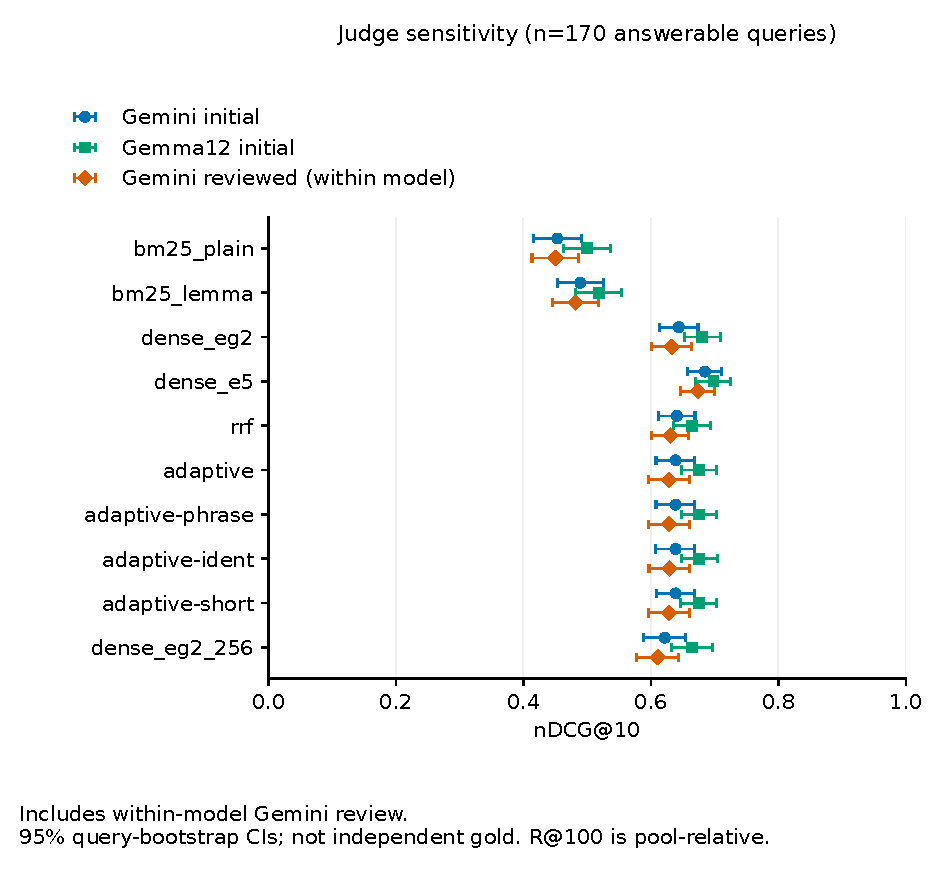
\includegraphics[width=\linewidth]{judge_sensitivity.pdf}
\caption{System scores and 95\% query-bootstrap intervals across relevance variants. Differences between separate intervals do not replace paired statistical comparisons.}
\label{fig:judge-sensitivity}
\end{figure}

\begin{figure}[p]
\centering
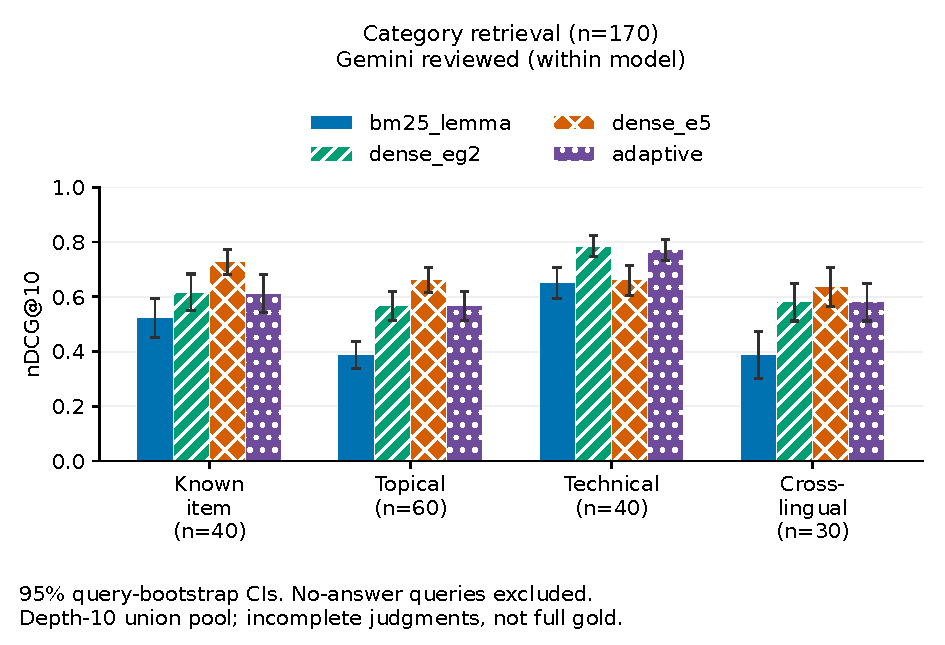
\includegraphics[width=\linewidth]{category_ndcg.pdf}
\caption{nDCG@10 by query category for four principal systems under the primary relevance variant. Each category uses its own query-bootstrap interval. No-answer queries are excluded.}
\label{fig:categories}
\end{figure}

\subsection{Controls}
\paragraph{Candidate universe.} E5 searches 4\,137 text documents; the full EG2 index holds 6\,054 documents, including media. Restricting EG2 to the same 4\,137 text documents (\sys{dense\_eg2\_text}) changes its nDCG@10 by $-0.0015$ under reviewed Gemini labels (0.633 to 0.631); 0.29\% of its top-10 documents were not in the judged pool. The paired difference EG2$_{\mathrm{text}}-{}$E5 is $-0.042$ nDCG@10 (95\% CI $-0.078$ to $-0.006$, unadjusted $p=0.018$) with reviewed Gemini labels and $-0.019$ ($-0.052$ to $0.014$, $p=0.26$) with Gemma~4 12B labels (Table~\ref{tab:encoder-control}). Thus the candidate restriction has a small point effect in this control, while statistical support for the encoder difference depends on the labels. These exploratory comparisons use unadjusted p-values and an incomplete judgement pool.

\begin{table}[p]
\centering
\caption{E5 against EG2 on the same 4\,137 text documents. $\Delta$ is the paired difference from E5 with a 95\% query-bootstrap interval and an unadjusted sign-flip $p$; unjudged documents count as non-relevant, and their share is shown.}
\label{tab:encoder-control}
% Generated from primary=gemini_reviewed; see ../manifest.json for source SHA-256.
\noindent\textbf{Gemini reviewed}
\par\smallskip
% E5 against EG2 on the same 4137 text documents; source encoder_control.json
\begingroup\small\setlength{\tabcolsep}{4pt}\renewcommand{\arraystretch}{1.3}
\noindent\begin{tabularx}{\linewidth}{@{}l*{4}{>{\centering\arraybackslash}X}@{}}
\toprule
System & nDCG@10 & $\Delta$ [95\% CI] vs E5 & p & Unjudged@10 \\
\midrule
\sys{dense\_e5} & 0.674 & -- & -- & 0.000 \\
\sys{dense\_eg2} & 0.633 & \shortstack{-0.041 \\ {\footnotesize[-0.077, -0.005]}} & 0.023 & 0.000 \\
\sys{dense\_eg2\_text} & 0.631 & \shortstack{-0.042 \\ {\footnotesize[-0.078, -0.006]}} & 0.018 & 0.003 \\
\bottomrule
\end{tabularx}\endgroup

\par\medskip
\noindent\textbf{Gemini initial}
\par\smallskip
% E5 against EG2 on the same 4137 text documents; source encoder_control.json
\begingroup\small\setlength{\tabcolsep}{4pt}\renewcommand{\arraystretch}{1.3}
\noindent\begin{tabularx}{\linewidth}{@{}l*{4}{>{\centering\arraybackslash}X}@{}}
\toprule
System & nDCG@10 & $\Delta$ [95\% CI] vs E5 & p & Unjudged@10 \\
\midrule
\sys{dense\_e5} & 0.685 & -- & -- & 0.000 \\
\sys{dense\_eg2} & 0.644 & \shortstack{-0.041 \\ {\footnotesize[-0.075, -0.007]}} & 0.020 & 0.000 \\
\sys{dense\_eg2\_text} & 0.642 & \shortstack{-0.042 \\ {\footnotesize[-0.077, -0.009]}} & 0.014 & 0.003 \\
\bottomrule
\end{tabularx}\endgroup

\par\medskip
\noindent\textbf{Gemma 12B initial}
\par\smallskip
% E5 against EG2 on the same 4137 text documents; source encoder_control.json
\begingroup\small\setlength{\tabcolsep}{4pt}\renewcommand{\arraystretch}{1.3}
\noindent\begin{tabularx}{\linewidth}{@{}l*{4}{>{\centering\arraybackslash}X}@{}}
\toprule
System & nDCG@10 & $\Delta$ [95\% CI] vs E5 & p & Unjudged@10 \\
\midrule
\sys{dense\_e5} & 0.698 & -- & -- & 0.000 \\
\sys{dense\_eg2} & 0.681 & \shortstack{-0.018 \\ {\footnotesize[-0.050, +0.015]}} & 0.285 & 0.000 \\
\sys{dense\_eg2\_text} & 0.680 & \shortstack{-0.019 \\ {\footnotesize[-0.052, +0.014]}} & 0.258 & 0.003 \\
\bottomrule
\end{tabularx}\endgroup

\end{table}

\paragraph{Whole-word coverage.} The adaptive rule's exact-phrase test counted substrings (Appendix~\ref{sec:intro-history}). With the corrected rule, the top~10 changes for one query of 200 in each adaptive variant, and adaptive nDCG@10 moves from 0.629 to 0.627 (reviewed Gemini), 0.639 to 0.637 (initial Gemini) and stays at 0.675 (Gemma~4 12B). The frozen primary results are retained; the corrected point score does not create an adaptive advantage over dense EG2.

\subsection{Judges}
Table~\ref{tab:judge-checks} reports grades over the whole pool and on two construction-based diagnostic subsets: pooled authored targets and designated no-answer pairs. These expectations are not independent human labels. Table~\ref{tab:judge-agreement} reports pairwise agreement. Gemini, the two Gemma models and GPT-6-Luna agree with linear-weighted $\kappa$ between 0.535 and 0.652. Gemini gives the target document of a known-item or other answerable query grade~2 in 85.8\% of the 134 pooled targets, Gemma~4 12B in 67.2\%: the larger Gemma model agrees best with Gemini overall but rarely gives full marks. On the 708 pooled pairs of no-answer queries, Gemini, Gemma~4 12B and Gemma~4 E4B give grade~0 in 90.4\%, 91.2\% and 93.5\% of pairs.

GPT-6-Luna, which wrote the queries, is the most lenient judge: its mean grade is 0.633 against 0.421--0.447 for the other judges, and it gives a positive grade to 24.3\% of the no-answer pairs, against 6.5--9.6\% for the others. Its grades are higher than every other judge's on average by 0.19--0.21. This is consistent with self-preference by the query author, but general leniency would produce the same pattern. The present comparison cannot distinguish those explanations. GPT grades are not used in any relevance label.

\begin{table}[p]
\centering
\caption{Judges on the 5\,572 pooled pairs: mean grade, grade counts, and construction-based checks (share of pooled answerable-query targets graded 2; share of pooled no-answer pairs graded 0).}
\label{tab:judge-checks}
% Generated from primary=gemini_reviewed; see ../manifest.json for source SHA-256.
% grades on the whole pool and known-answer checks; source judges.json
\begingroup\small\setlength{\tabcolsep}{4pt}\renewcommand{\arraystretch}{1.3}
\noindent\begin{tabularx}{\linewidth}{@{}l*{5}{>{\centering\arraybackslash}X}@{}}
\toprule
Judge & Pairs & Mean grade & 0 / 1 / 2 & Target = 2, \% & No-answer = 0, \% \\
\midrule
Gemini 3.8 Flash & 5\,572 & 0.421 & 3\,522 / 1\,756 / 294 & 85.8 (n=134) & 90.4 (n=708) \\
Gemma 4 12B & 5\,572 & 0.447 & 3\,316 / 2\,024 / 232 & 67.2 (n=134) & 91.2 (n=708) \\
Gemma 4 E4B & 5\,572 & 0.438 & 3\,519 / 1\,665 / 388 & 74.6 (n=134) & 93.5 (n=708) \\
GPT-6-Luna & 5\,572 & 0.633 & 2\,554 / 2\,510 / 508 & 91.8 (n=134) & 75.7 (n=708) \\
\bottomrule
\end{tabularx}\endgroup

\end{table}

\begin{table}[p]
\centering
\caption{Pairwise agreement between judges on the same 5\,572 pairs: linear-weighted Cohen's $\kappa$ with a 95\% interval from 2\,000 query-level bootstrap resamples, exact agreement, and the mean grade difference.}
\label{tab:judge-agreement}
% Generated from primary=gemini_reviewed; see ../manifest.json for source SHA-256.
% linear-weighted kappa, CI by resampling queries; source judges.json
\begingroup\small\setlength{\tabcolsep}{4pt}\renewcommand{\arraystretch}{1.3}
\noindent\begin{tabularx}{\linewidth}{@{}l*{4}{>{\centering\arraybackslash}X}@{}}
\toprule
Judges & Pairs & Weighted $\kappa$ [95\% CI] & Exact agreement & Mean A$-$B \\
\midrule
Gemini 3.8 Flash – Gemma 4 12B & 5\,572 & 0.652 [0.625, 0.677] & 0.804 & -0.026 \\
Gemini 3.8 Flash – Gemma 4 E4B & 5\,572 & 0.591 [0.559, 0.622] & 0.768 & -0.017 \\
Gemini 3.8 Flash – GPT-6-Luna & 5\,572 & 0.621 [0.595, 0.644] & 0.759 & -0.212 \\
Gemma 4 12B – Gemma 4 E4B & 5\,572 & 0.650 [0.625, 0.674] & 0.799 & +0.008 \\
Gemma 4 12B – GPT-6-Luna & 5\,572 & 0.586 [0.559, 0.612] & 0.741 & -0.186 \\
Gemma 4 E4B – GPT-6-Luna & 5\,572 & 0.535 [0.506, 0.564] & 0.700 & -0.195 \\
\bottomrule
\end{tabularx}\endgroup

\end{table}

\subsection{Images and speech}
Table~\ref{tab:multimodal} reports separate image-caption and speech-transcript retrieval tasks. These point estimates have no computed confidence intervals. The monolingual text-only speech condition uses the same transcript as query and indexed text, so it is a ceiling condition rather than a realistic paraphrased-query evaluation. Cross-language queries are parallel source transcripts and also do not represent arbitrary conversational audio search.

\begin{table}[p]
\centering
\caption{Separate source-labelled multimodal tasks: query and candidate counts, followed by point estimates. No confidence intervals are fabricated. Speech text mode indexes the transcript; both mode combines transcript and audio.}
\label{tab:multimodal}
% Generated from primary=gemini_reviewed; see ../manifest.json for source SHA-256.
% Separate multimodal tasks; confidence intervals unavailable in source (not fabricated).
\begingroup\small\setlength{\tabcolsep}{4pt}\renewcommand{\arraystretch}{1.3}
\noindent\begin{tabularx}{\linewidth}{@{}l*{2}{>{\centering\arraybackslash}X}@{}}
\toprule
Mode & Queries & Items \\
\midrule
Image / ru & 1000 & 1000 \\
Image / uk & 1000 & 1000 \\
Speech / ru->ru / audio & 265 & 400 \\
Speech / ru->ru / both & 265 & 400 \\
Speech / ru->ru / text & 265 & 400 \\
Speech / ru->uk / audio & 194 & 400 \\
Speech / ru->uk / both & 194 & 400 \\
Speech / ru->uk / text & 194 & 400 \\
Speech / uk->ru / audio & 194 & 400 \\
Speech / uk->ru / both & 194 & 400 \\
Speech / uk->ru / text & 194 & 400 \\
Speech / uk->uk / audio & 262 & 400 \\
Speech / uk->uk / both & 262 & 400 \\
Speech / uk->uk / text & 262 & 400 \\
\bottomrule
\end{tabularx}\endgroup

\par\medskip
% Point estimates only; confidence intervals unavailable. Recall is task-specific.
\begingroup\small\setlength{\tabcolsep}{4pt}\renewcommand{\arraystretch}{1.3}
\noindent\begin{tabularx}{\linewidth}{@{}l*{4}{>{\centering\arraybackslash}X}@{}}
\toprule
Mode & recall@1 & recall@5 & recall@10 & mrr \\
\midrule
Image / ru & 0.889 & 0.983 & 0.994 & 0.932 \\
Image / uk & 0.857 & 0.977 & 0.986 & 0.909 \\
Speech / ru->ru / audio & 0.996 & 1.000 & 1.000 & 0.997 \\
Speech / ru->ru / both & 1.000 & 1.000 & 1.000 & 1.000 \\
Speech / ru->ru / text & 1.000 & 1.000 & 1.000 & 1.000 \\
Speech / ru->uk / audio & 0.985 & 1.000 & 1.000 & 0.991 \\
Speech / ru->uk / both & 1.000 & 1.000 & 1.000 & 1.000 \\
Speech / ru->uk / text & 1.000 & 1.000 & 1.000 & 1.000 \\
Speech / uk->ru / audio & 0.985 & 1.000 & 1.000 & 0.990 \\
Speech / uk->ru / both & 1.000 & 1.000 & 1.000 & 1.000 \\
Speech / uk->ru / text & 1.000 & 1.000 & 1.000 & 1.000 \\
Speech / uk->uk / audio & 0.996 & 1.000 & 1.000 & 0.997 \\
Speech / uk->uk / both & 1.000 & 1.000 & 1.000 & 1.000 \\
Speech / uk->uk / text & 1.000 & 1.000 & 1.000 & 1.000 \\
\bottomrule
\end{tabularx}\endgroup

\end{table}

\subsection{Latency and indexing cost}
\ifpaperlatency
Table~\ref{tab:latency} reports warm per-query latency on the same 200 queries. These are evaluation-harness timings on one laptop, not interactive response-time guarantees. The models remain loaded between systems: the device-wide GPU-memory increase from each baseline is not an isolated footprint for that system.
\begin{table}[p]
\centering
\caption{Warm query latency in milliseconds: p50 and p95 on GPU and CPU. VRAM is the device-wide increase above the stage baseline; previously loaded models remain resident.}
\label{tab:latency}
% Generated from primary=gemini_reviewed; see ../manifest.json for source SHA-256.
% per-query latency in ms (query embedding and chunk search; document collapse excluded); source efficiency.json
\begingroup\small\setlength{\tabcolsep}{4pt}\renewcommand{\arraystretch}{1.3}
\noindent\begin{tabularx}{\linewidth}{@{}l*{5}{>{\centering\arraybackslash}X}@{}}
\toprule
System & GPU p50 & GPU p95 & CPU p50 & CPU p95 & VRAM +MiB \\
\midrule
\sys{bm25\_plain} & 12.3 & 41.6 & 13.8 & 48.0 & 0 \\
\sys{bm25\_lemma} & 19.9 & 64.1 & 19.9 & 62.4 & 0 \\
\sys{dense\_eg2} & 137.9 & 189.4 & 218.3 & 261.5 & 1592 \\
\sys{dense\_eg2\_256} & 67.2 & 79.5 & 185.8 & 212.9 & 0 \\
\sys{dense\_e5} & 93.1 & 117.1 & 217.2 & 254.5 & 2130 \\
\sys{rrf} & 132.5 & 177.4 & 266.8 & 362.1 & 2 \\
\sys{adaptive} & 134.7 & 186.7 & 230.4 & 286.3 & 0 \\
\bottomrule
\end{tabularx}\endgroup

\end{table}
\begin{figure}[p]
\centering
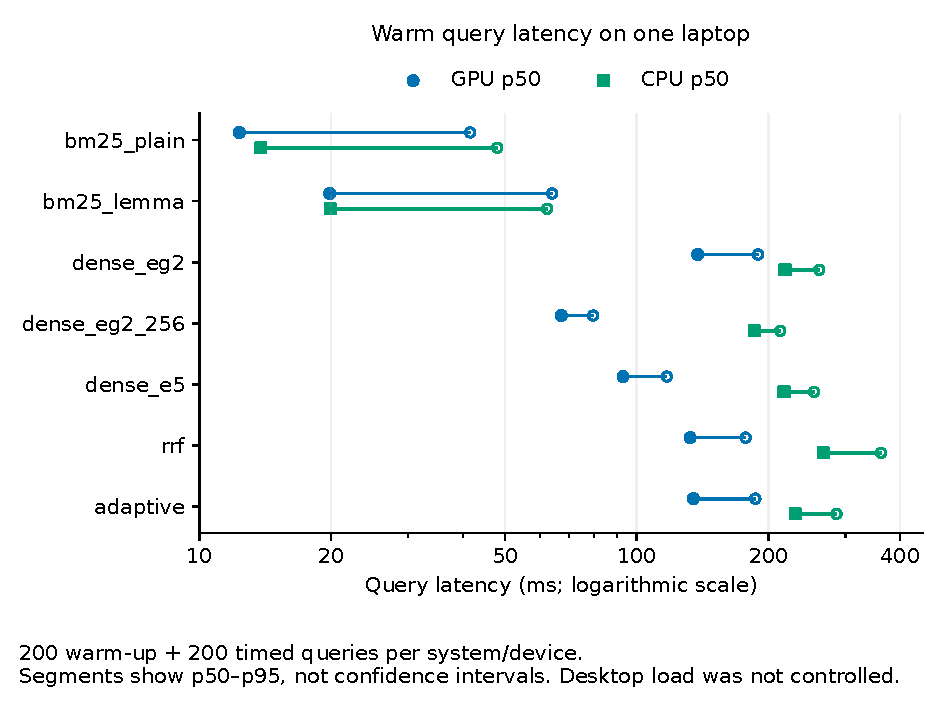
\includegraphics[width=\linewidth]{query_latency.pdf}
\caption{Query latency after a full warm-up. Markers show p50 and open endpoints p95, not confidence limits; the horizontal axis is logarithmic. Both passes include all 200 queries.}
\label{fig:query-latency}
\end{figure}

\begin{figure}[p]
\centering
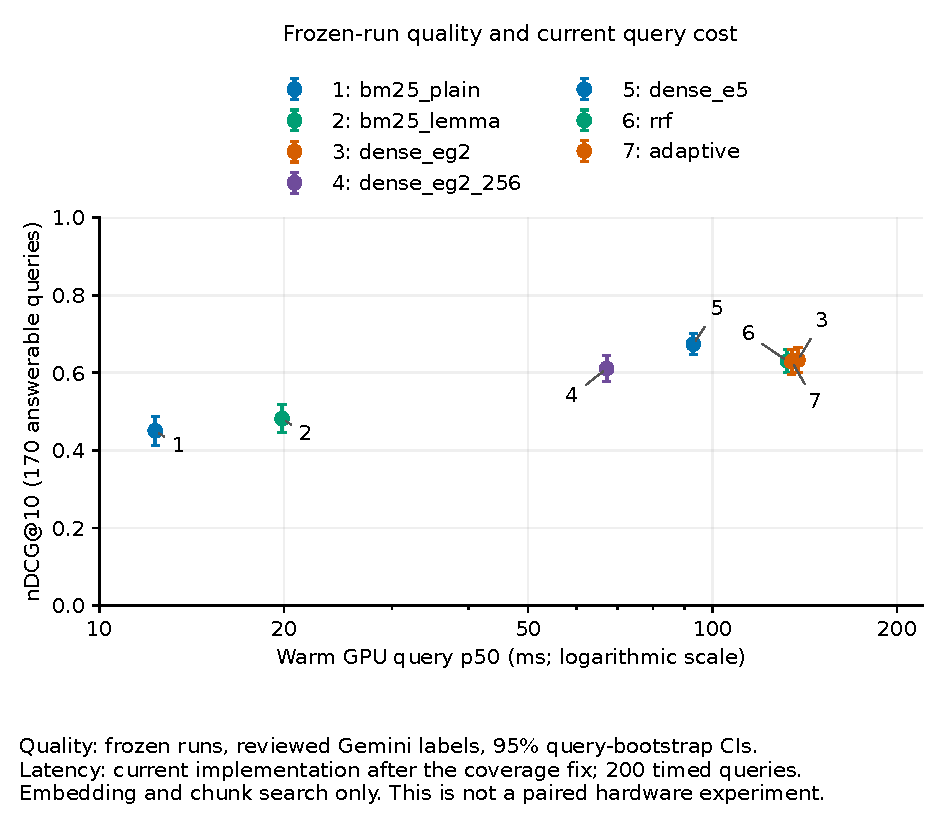
\includegraphics[width=\linewidth]{latency_quality.pdf}
\caption{Frozen original-run quality against current warm GPU query cost. Quality intervals use 170 answerable queries and reviewed Gemini labels; latency uses all 200 queries after the whole-word coverage correction. The two axes describe different code revisions, as disclosed in the control analysis, and do not form a paired hardware experiment. Document collapse is excluded from the timer.}
\label{fig:latency-quality}
\end{figure}
\else
\pending{Complete CPU/GPU query latency}
\fi
\ifpaperindexing
Table~\ref{tab:indexing} reports the GPU sample of 475 files and CPU sample of 95 files. Their compositions differ; chunks per second are descriptive throughput figures, and the ratio of wall times is not a paired hardware speedup.
\begin{table}[p]
\centering
\caption{Indexing into an empty database on two differently sized fixed samples. Counts refer to the files selected and chunks produced; RSS is the child-process peak. Sample disk includes database sidecars; full-index sizes count the main database files.}
\label{tab:indexing}
% Generated from primary=gemini_reviewed; see ../manifest.json for source SHA-256.
% indexing a fixed sample of the corpus with the archive CLI; source efficiency.json
\begingroup\small\setlength{\tabcolsep}{4pt}\renewcommand{\arraystretch}{1.3}
\noindent\begin{tabularx}{\linewidth}{@{}l*{7}{>{\centering\arraybackslash}X}@{}}
\toprule
Device & Files & Chunks & Seconds & Chunks/s & DB MiB & RSS MiB & VRAM +MiB \\
\midrule
GPU & 475 & 5\,155 & 106.1 & 48.58 & 59.9 & 2591 & 6816 \\
CPU & 95 & 1\,187 & 1395.1 & 0.85 & 13.6 & 2979 & 0 \\
\bottomrule
\end{tabularx}\endgroup

\par\medskip
% main database files; sample disk above includes sidecars
\begingroup\small\setlength{\tabcolsep}{4pt}\renewcommand{\arraystretch}{1.3}
\noindent\begin{tabularx}{\linewidth}{@{}l*{1}{>{\centering\arraybackslash}X}@{}}
\toprule
Full index & Main database MiB \\
\midrule
e5.sqlite3 & 1096.4 \\
full.sqlite3 & 1120.7 \\
noshort.sqlite3 & 1208.5 \\
plain.sqlite3 & 1094.7 \\
\bottomrule
\end{tabularx}\endgroup

\end{table}
\else
\pending{Complete CPU/GPU indexing measurements}
\fi

\subsection{Quantized retrieval}
\ifpapergguf
\begin{table}[p]
\centering
\caption{GGUF EG2 builds on the same text candidates as the bfloat16 reference. Query latency follows a full 200-query warm-up. Differences use reviewed Gemini labels and exploratory unadjusted paired tests; unjudged results are counted as non-relevant. File sizes are MiB.}
\label{tab:gguf}
% Generated from primary=gemini_reviewed; see ../manifest.json for source SHA-256.
% dense EG2 on the 4137 text documents; labels gemini_reviewed; source efficiency.json quantization
\begingroup\small\setlength{\tabcolsep}{4pt}\renewcommand{\arraystretch}{1.3}
\noindent\begin{tabularx}{\linewidth}{@{}l*{3}{>{\centering\arraybackslash}X}@{}}
\toprule
Build & File MiB & Chunks/s & Query p50 \\
\midrule
bf16 (SentenceTransformers) & -- & -- & -- \\
f16 & 532 & 46 & 76.7 \\
Q8\_0 & 296 & 48 & 86.0 \\
Q4\_K\_M & 173 & 46 & 83.6 \\
\bottomrule
\end{tabularx}\endgroup

\par\medskip
% dense EG2 on the 4137 text documents; labels gemini_reviewed; source efficiency.json quantization
\begingroup\small\setlength{\tabcolsep}{4pt}\renewcommand{\arraystretch}{1.3}
\noindent\begin{tabularx}{\linewidth}{@{}l*{4}{>{\centering\arraybackslash}X}@{}}
\toprule
Build & nDCG@10 & $\Delta$ [95\% CI] & p & Unjudged@10 \\
\midrule
bf16 (SentenceTransformers) & 0.631 & -- & -- & 0.003 \\
f16 & 0.631 & \shortstack{-0.001 \\ {\footnotesize[-0.005, +0.003]}} & 0.734 & 0.016 \\
Q8\_0 & 0.630 & \shortstack{-0.002 \\ {\footnotesize[-0.006, +0.003]}} & 0.504 & 0.018 \\
Q4\_K\_M & 0.613 & \shortstack{-0.018 \\ {\footnotesize[-0.030, -0.006]}} & 0.002 & 0.099 \\
\bottomrule
\end{tabularx}\endgroup

\par\medskip
% dense EG2 on the 4137 text documents; labels gemini_reviewed; source efficiency.json quantization; unjudged documents removed before ranking evaluation
\begingroup\small\setlength{\tabcolsep}{4pt}\renewcommand{\arraystretch}{1.3}
\noindent\begin{tabularx}{\linewidth}{@{}l*{3}{>{\centering\arraybackslash}X}@{}}
\toprule
Build & Condensed nDCG@10 & $\Delta$ [95\% CI] & p \\
\midrule
bf16 (SentenceTransformers) & 0.632 & -- & -- \\
f16 & 0.634 & \shortstack{+0.002 \\ {\footnotesize[-0.002, +0.006]}} & 0.297 \\
Q8\_0 & 0.633 & \shortstack{+0.000 \\ {\footnotesize[-0.004, +0.005]}} & 0.869 \\
Q4\_K\_M & 0.636 & \shortstack{+0.004 \\ {\footnotesize[-0.007, +0.015]}} & 0.454 \\
\bottomrule
\end{tabularx}\endgroup

\end{table}
\begin{figure}[p]
\centering
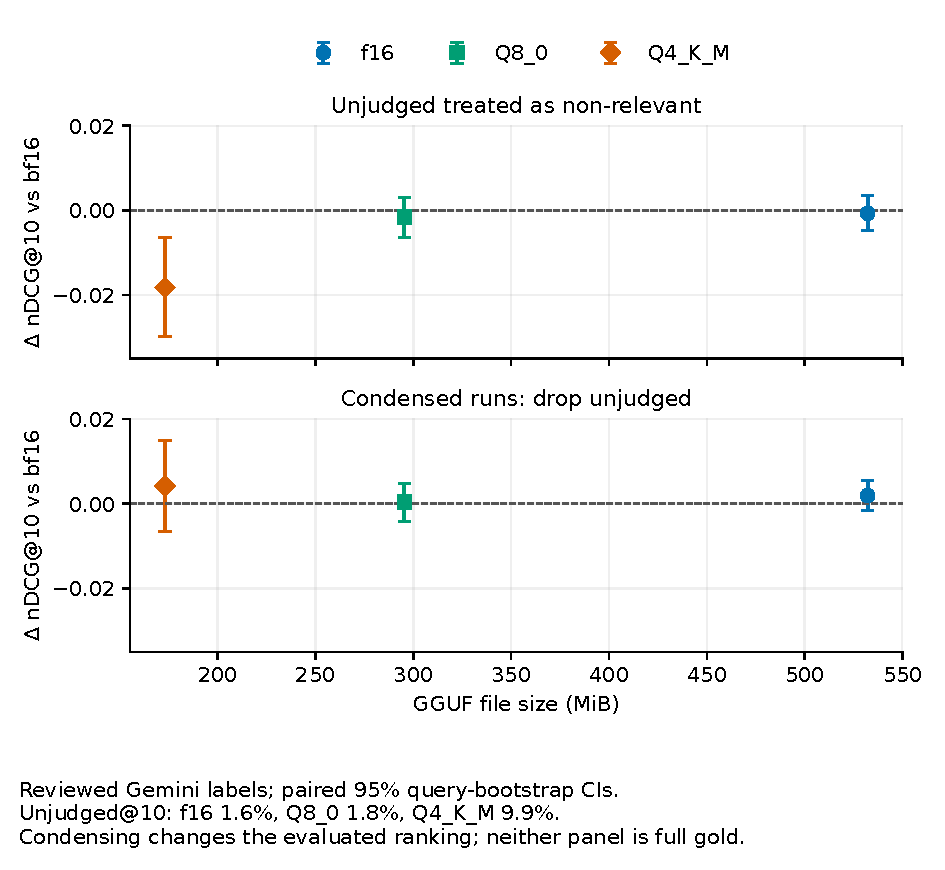
\includegraphics[width=\linewidth]{quantization_quality.pdf}
\caption{Paired nDCG@10 differences from bf16 EG2 versus GGUF file size on identical text candidates. The upper panel treats unjudged documents as non-relevant; the lower panel removes them. Error bars are 95\% query-bootstrap intervals. The dependence on judgement coverage prevents interpreting the upper Q4 difference as an isolated quantization effect.}
\label{fig:quantization-quality}
\end{figure}
Table~\ref{tab:gguf} reports retrieval quality, embedding throughput and local-server query latency. The separate cosine-reference experiment in the appendix does not substitute for these retrieval comparisons. The f16 and Q8 point differences from the bf16 reference are small, but intervals containing zero do not establish equivalence. For Q4, treating unjudged results as non-relevant gives a difference of $-0.018$ (95\% CI $[-0.030,-0.006]$); 9.9\% of its top-ten results are unjudged, compared with 0.3\% for the reference. On condensed runs the Q4 difference is $+0.004$ with an interval spanning zero. Removing unjudged results changes the evaluated ranking; it does not establish their relevance. Thus the frozen pool does not identify an intrinsic Q4 quality loss. These comparisons also change backend and numerical precision, not only quantization.
\else
\pending{GGUF retrieval-quality experiment incomplete; reference cosine measurements are in the appendix}
\fi

\subsection{Synthetic scaling}
\ifpaperann
\begin{table}[p]
\centering
\caption{Exact and approximate search on synthetic collections derived from the real vectors. Latencies are p50 milliseconds for a single query. HNSW cells show latency / recall@10 against exact search; construction time is seconds. This experiment measures chunk-vector search only.}
\label{tab:ann}
% Generated from primary=gemini_reviewed; see ../manifest.json for source SHA-256.
% p50 ms per single query; HNSW cells: p50 ms / strict-ID recall@10 against exact; source ann_scaling.json
\begingroup\small\setlength{\tabcolsep}{4pt}\renewcommand{\arraystretch}{1.3}
\noindent\begin{tabularx}{\linewidth}{@{}l*{5}{>{\centering\arraybackslash}X}@{}}
\toprule
Vectors & NumPy top-k & Faiss flat & HNSW build s & HNSW ef64 & HNSW ef256 \\
\midrule
100\,000 & 6.16 & 10.65 & 9 & 0.19 / 0.914 & 0.57 / 0.984 \\
300\,000 & 17.85 & 26.52 & 33 & 0.27 / 0.940 & 0.69 / 0.990 \\
1\,000\,000 & 51.78 & 75.83 & 187 & 0.29 / 0.904 & 0.97 / 0.991 \\
2\,000\,000 & 106.63 & 139.95 & 676 & 0.39 / 0.893 & 1.28 / 0.983 \\
\bottomrule
\end{tabularx}\endgroup

\par\medskip
% Actual semantic_scored path with candidate gather, full sort, pool400; no database polling; flat exact agreement / fraction at reference kth score within1e-6; source ann_reference_audit.json
\begingroup\small\setlength{\tabcolsep}{4pt}\renewcommand{\arraystretch}{1.3}
\noindent\begin{tabularx}{\linewidth}{@{}l*{3}{>{\centering\arraybackslash}X}@{}}
\toprule
Vectors & Archive path p50 ms & Flat ID agreement & Flat score threshold \\
\midrule
100\,000 & 60.84 & 1.000 & 1.000 \\
300\,000 & 166.80 & 1.000 & 1.000 \\
1\,000\,000 & 497.64 & 1.000 & 1.000 \\
2\,000\,000 & 2441.83 & 1.000 & 1.000 \\
\bottomrule
\end{tabularx}\endgroup

\par\smallskip
At 2\,000\,000 vectors, observed p50 is 106.6 ms for optimized NumPy top-k and 2441.8 ms for the archive vector path. HNSW ef256 is 1.28 ms at strict-ID recall@10 0.9825. These are sequential desktop-session measurements of different algorithms and output pools (10 versus 400), not paired hardware speedups or end-to-end interface latency.

\end{table}
\begin{figure}[p]
\centering
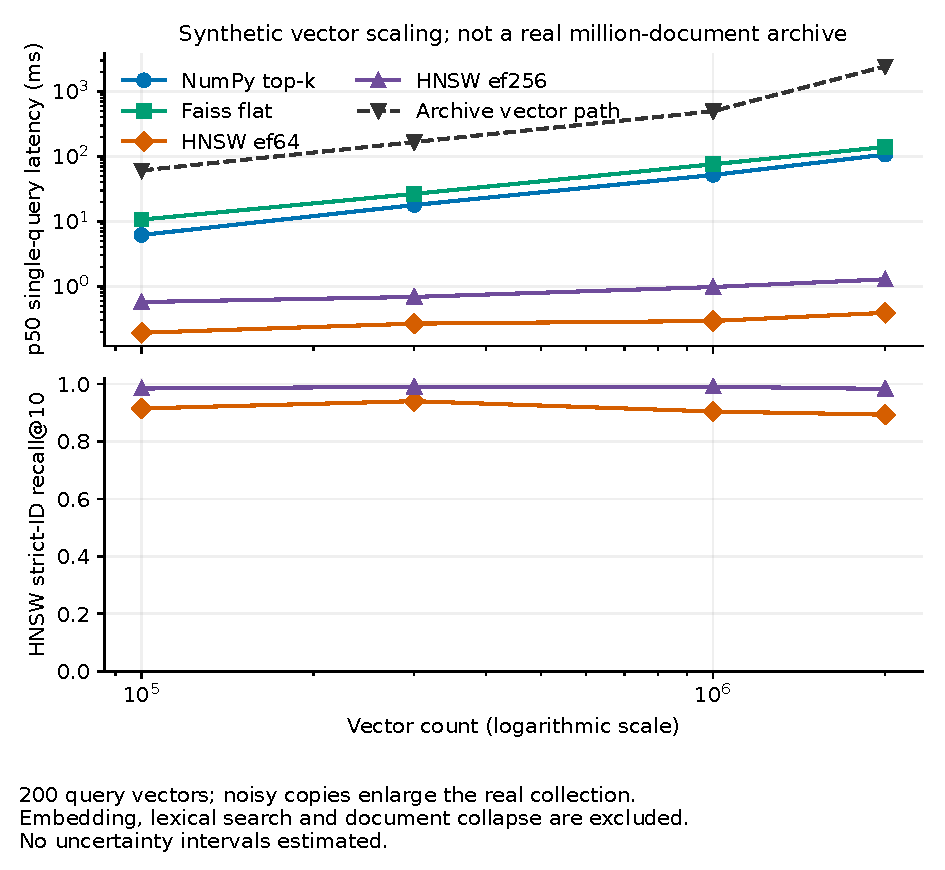
\includegraphics[width=\linewidth]{ann_scaling.pdf}
\caption{Vector-search latency and HNSW recall on synthetic enlarged collections. The latency axis is logarithmic, and no uncertainty intervals are estimated.}
\label{fig:ann-scaling}
\end{figure}
Table~\ref{tab:ann} separates exact vector-search cost from HNSW approximation. It excludes query embedding, lexical search and document collapse, and does not measure retrieval relevance on a real million-document archive.
\else
\pending{Complete exact/Faiss/HNSW scaling experiment}
\fi

\subsection{Additional target types}\label{sec:results-extension}
\ifpaperextension
The separate extension uses 50 Qwen-written queries targeting 20 documents, 15 tables and 15 repository files, evaluated with the corrected coverage rule. Initial Gemini labels and initial Gemma~4 12B labels are reported separately in Table~\ref{tab:extension}. The 50 records contain 49 distinct query wordings; one wording targets two files. They are not mixed into the original 200 or its primary relevance labels. GPT is comparison-only. Differences between the two query populations cannot identify self-preference because authorship, target type and difficulty also differ.
\begin{table}[p]
\centering
\caption{nDCG@10 and 95\% query-bootstrap intervals on the separate 50-query extension. Both label variants are initial assessments; neither is the original benchmark's reviewed primary variant.}
\label{tab:extension}
% Generated from primary=gemini_reviewed; see ../manifest.json for source SHA-256.
% nDCG@10, 95% query-bootstrap CI; separate 50-query extension; source extension.json
\begingroup\small\setlength{\tabcolsep}{4pt}\renewcommand{\arraystretch}{1.3}
\noindent\begin{tabularx}{\linewidth}{@{}l*{2}{>{\centering\arraybackslash}X}@{}}
\toprule
System & Gemini initial & Gemma 12B initial \\
\midrule
bm25\_plain & \shortstack{0.496 \\ {\footnotesize[0.404, 0.590]}} & \shortstack{0.507 \\ {\footnotesize[0.409, 0.604]}} \\
bm25\_lemma & \shortstack{0.523 \\ {\footnotesize[0.431, 0.617]}} & \shortstack{0.540 \\ {\footnotesize[0.443, 0.639]}} \\
dense\_eg2 & \shortstack{0.759 \\ {\footnotesize[0.697, 0.817]}} & \shortstack{0.769 \\ {\footnotesize[0.701, 0.832]}} \\
dense\_e5 & \shortstack{0.721 \\ {\footnotesize[0.654, 0.785]}} & \shortstack{0.730 \\ {\footnotesize[0.666, 0.790]}} \\
rrf & \shortstack{0.684 \\ {\footnotesize[0.619, 0.749]}} & \shortstack{0.696 \\ {\footnotesize[0.623, 0.766]}} \\
adaptive & \shortstack{0.756 \\ {\footnotesize[0.694, 0.814]}} & \shortstack{0.765 \\ {\footnotesize[0.697, 0.827]}} \\
adaptive-phrase & \shortstack{0.756 \\ {\footnotesize[0.694, 0.814]}} & \shortstack{0.765 \\ {\footnotesize[0.697, 0.827]}} \\
adaptive-ident & \shortstack{0.756 \\ {\footnotesize[0.694, 0.814]}} & \shortstack{0.765 \\ {\footnotesize[0.697, 0.827]}} \\
adaptive-short & \shortstack{0.756 \\ {\footnotesize[0.694, 0.814]}} & \shortstack{0.765 \\ {\footnotesize[0.697, 0.827]}} \\
dense\_eg2\_256 & \shortstack{0.713 \\ {\footnotesize[0.639, 0.782]}} & \shortstack{0.732 \\ {\footnotesize[0.662, 0.797]}} \\
\bottomrule
\end{tabularx}\endgroup

\end{table}

With initial Gemini labels, EG2 scores 0.759, adaptive fusion 0.756 and E5 0.721, compared with 0.523 for lemmatized BM25. With initial Gemma~4 12B labels the corresponding scores are 0.769, 0.765, 0.730 and 0.540. Adaptive exceeds both lexical baselines after Holm correction in both label variants; neither EG2 nor E5 is separated from adaptive by those tests. The changed point order of the dense encoders is cohort-specific evidence, not a comparison of overall difficulty with the original benchmark. GPT remains the most lenient judge on Qwen-written queries as well (mean grade 0.550 versus 0.379 for Gemini and 0.437 for Gemma), reinforcing that the initial GPT pattern does not identify query-author self-preference.

\ifpaperextensionunique
Keeping the lowest query ID per normalized wording removes q249, without selecting by retrieval score. Table~\ref{tab:extension-unique} reports this exploratory sensitivity. The 50-record intervals treat records as resampling units despite their shared wording; the separate sensitivity avoids that duplicate but does not make the sample representative.
\begin{table}[p]
\centering
\caption{Five principal systems on the unique-wording subset of the extension. Initial labels and query-bootstrap intervals; remaining systems and paired statistics are preserved in the result JSON.}
\label{tab:extension-unique}
% Generated from primary=gemini_reviewed; see ../manifest.json for source SHA-256.
Unique-wording sensitivity: 49 queries.
\par\smallskip
% keep lowest qid per normalized wording; source extension.json
\begingroup\small\setlength{\tabcolsep}{4pt}\renewcommand{\arraystretch}{1.3}
\noindent\begin{tabularx}{\linewidth}{@{}l*{2}{>{\centering\arraybackslash}X}@{}}
\toprule
System & Gemini initial & Gemma 12B initial \\
\midrule
bm25\_plain & \shortstack{0.503 \\ {\footnotesize[0.407, 0.597]}} & \shortstack{0.513 \\ {\footnotesize[0.414, 0.611]}} \\
bm25\_lemma & \shortstack{0.530 \\ {\footnotesize[0.439, 0.624]}} & \shortstack{0.546 \\ {\footnotesize[0.448, 0.646]}} \\
dense\_e5 & \shortstack{0.717 \\ {\footnotesize[0.649, 0.782]}} & \shortstack{0.724 \\ {\footnotesize[0.659, 0.786]}} \\
dense\_eg2 & \shortstack{0.757 \\ {\footnotesize[0.695, 0.813]}} & \shortstack{0.765 \\ {\footnotesize[0.698, 0.826]}} \\
adaptive & \shortstack{0.754 \\ {\footnotesize[0.692, 0.810]}} & \shortstack{0.760 \\ {\footnotesize[0.694, 0.821]}} \\
\bottomrule
\end{tabularx}\endgroup

\end{table}
\fi

\else
\pending{Separate 50-query document/table/code extension and its relevance assessments}
\fi
